
\chapter{Hardware Design} % Main chapter title

\label{Chapter3} % For referencing the chapter elsewhere, use \ref{Chapter1} 

\lhead{Chapter 3. \emph{Hardware Design}} % This is for the header on each page - perhaps a shortened title

There are two hardware components required for fingerprinting: the fingerprinting unit itself and the centralized comparator. The fingerprint unit must passively monitor the data bus of a core to compute fingerprints and periodically send these fingerprints to the comparator. The comparator must pool and organize fingerprints collected from all the cores and compare them to decide if the system is operating correctly. The comparator must then notify the monitor core upon the successful completion of a task or if an error has been detected. Three interfaces must be specified: the cores to the fingerprint unit, the fingerprint unit to the comparator, and the comparator to the monitor. This section will describe these interfaces as well as cover the mechanism by which rate monotonic (RM) scheduling is supported (i.e. preemption of fingerprinted tasks) and the internal microarchitectures of the fingerprint unit and the comparator.

\section{Fingerprinting Interfaces}
\subsection{Processor/Fingerprint Unit Interface}
Table \ref{t:fprint_reg} contains the list of registers in the fingerprint unit that can be written by the processor it is attached to. Note that all address offsets are given from the perspective of the sender. The sender address offset is always shifted left by two bits compared to the offset the receiver uses. The current state register bitfield is defined in Table \ref{t:cs_bitfield}.
\begin{table}
\centering
    \begin{tabular}{| l | l | l  | p{6cm} |}
    \hline
    Register & RW & Offset & Function\\ \hline
    Current State (CS) & W & 0x0 & Used to enable and disable fingerprinting\\ \hline
    Block size (BS) & RW & 0x10 & The BS register contains the size of a fingerprinting block for the current task\\ \hline
    Pause  & R & 0x8 & The pause register is used by the interrupt trap to signal that the current task should pause its fingerprinting. The value read has no meaning.\\ \hline
    Unpause & R & 0xc & The unpause register is used by the interrupt trap to signal that the most recently paused task should resume fingerprinting. The value read has no meaning.\\ \hline
    \end{tabular}
    \caption{Fingerprint unit control registers}
    \label{t:fprint_reg}
\end{table}


\begin{table}
\centering
    \begin{tabular}{| l | l | l | p{6cm} |}
    \hline
    Name & Offset & Size(bits) & Function\\ \hline
    FID & 0x0 & 4 & The FID of the task beginning or ending fingerprinting.\\ \hline
    Enable bit & 0x4 & 1 & The enable bit signals whether fingerprinting is beginning or ending.\\ \hline
    \end{tabular}
    \caption{Current state register bitfield.}
    \label{t:cs_bitfield}
\end{table}

The functions used for this purpose are:
\begin{itemize}
\item{enable\_fprint\_task(int FID): begin fingerprinting on the given core a task with FID.} 
\item{disable\_fprint\_task(int FID): end fingerprinting on the given core a task with FID.}
\item{fprint\_set\_block\_size(int size): set the block size for the task beginning fingerprinting. Set prior to enabling fingerprinting.}
\end{itemize}

\emph{Block size:} A default value of 0xFFF is currently provided for the fingerprint unit. The block size \emph{MUST} be odd to function correctly. In anticipation of future work exploring the fingerprinting of both store and load instructions, the counter is currently set to increment by 2 since load instructions contribute half as many bits as store instructions (only the address is used). A value of 0xFFF = 4095 signifies that 2048 stores will be used to calculate a fingerprint. Each store contains 59 bits (27 address and 32 data bits). This means that each 32 bit fingerprint compresses 120832 bits of execution stream resulting in 3776x compression. A table of polynomials including block sizes over which a given hamming distance is achieved is provided in \cite{koopman200232}.
\begin{figure}
\centering
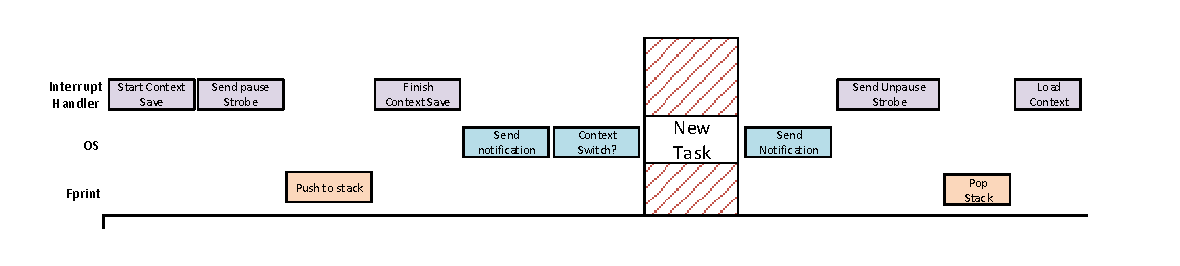
\includegraphics[scale=0.8]{Figures/interrupt}
\caption[Preemption of a fingerprinted task]{Preempting a fingerprinted task without corrupting the fingerprint. The low level assembly interrupt handler and the OS interrupt wrappers are depicted separately.}
\label{f:int}
\end{figure}
\emph{Pausing: } 	At times it may be necessary for one critical task to preempt another. 
	In the context of fingerprinting, this presents additional challenges:
		the fingerprinting of the preempted task must not be disrupted, but the fingerprinting logic must be available for the new task.
	Figure \ref{f:int} shows the procedure.
	First, the interrupt vector responsible for context saving located in the BSP is modified to send a strobe to the fingerprint unit notifying it that it should stop fingerprinting.



	The problem arises that there is no way for communication between software and hardware to occur without the software corrupting its own context (it must load the address of the hardware into a register). 
	We propose a convention whereby the fingerprinting hardware is able to roll back its calculations by one iteration, thus allowing a single store instruction to be executed without corrupting the fingerprint. 
	When an interrupt occurs, the initial context saving assembly routine is modified to store exactly one register onto the stack, and then this register is used to load the address of the fingerprint unit pause strobe (Listing \ref{l:int_trap_st}). 
	
		\begin{lstlisting}[frame=single,language=C,label=l:int_trap_st,caption=The updated trap at the start of an interrupt.]
stw   ra,  0(sp)
movhi ra,  \%hi(0x8100000)
ori   ra,  ra, 8
ldw   ra,    0(ra)
stw   r1,   8(sp)
stw   r2,  12(sp)
...
\end{lstlisting}

	The fingerprint unit rolls back its calculation by one iteration when it receives the pause strobe. 
	Following this, the RTOS has its own interrupt wrapper functions. The OS notifies the fingerprint unit that it is about to call the context switch routine.
	If a higher priority task is ready, then it will execute in its entirety.
	When the context switch function finally returns, the OS again sends another notification to the fingerprint unit. 
	Finally an unpause strobe is included in the context restore vector in the BSP (Listing \ref{l:int_trap_ld}).
	\begin{lstlisting}[frame=single,language=C,label=l:int_trap_ld,caption=The updated trap at the end of an interrupt.]
movhi ra,  %hi(0x8100000)
ori   ra,  ra, 12
ldw   ra,    0(ra)
ldw   r5,  68(sp)
ldw   ea,  72(sp)  
ldw   ra,   0(sp)
...
\end{lstlisting} 
	The main purpose of the OS notification is to guard against unwanted behaviours that may arise due to nested interrupts. It is possible to imagine other types of communication passing between the OS and the fingerprinting unit once fingerprinting has been successfully paused. 
	For instance, the fingerprinting unit currently only supports rate monotonic scheduling and stores paused task context on a stack. 
	It is reasonable for the OS to pass messages to the fingerprinting to notify it which task is being resumed and for the hardware stack to be replaced by a more flexible data structure. 
	There are potential issues here in that the unreliable core is now passing information to the FP unit that may affect the fingerprinting of several tasks if it is not done properly. 
	We do not explore this issue in any greater detail but note that this behaviour is easily supported by the hardware should it be desired.
%
%
%
%Corrupting the context is not an issue at the end of the interrupt. The unpause strobe can simply be activated before loading back the original context. It must be the case that no interrupt related stores occur after the unpause strobe. If stack exceptions are enabled, for instance, the location of the pause strobe would have to be slightly altered. Listing \ref{l:int_trap_ld} shows the unpause strobe in the trap.
%
%
%The last thing that should be mentioned with respect to pausing is that there is also a uCOS wrapper that is executed prior to the user defined interrupt handler. This can be modified in future versions to send more information from the OS to the fingerprinting unit about the task to be resumed. Figure \ref{f:exception_flow} shows the software flow of exception handling in the Nios system. Once fingerprinting is paused, the OS Interrupt Exit function can be modified to send more details to the fingerprinting unit using as of yet unspecified control registers.

%\begin{figure}[h]
%\centering
%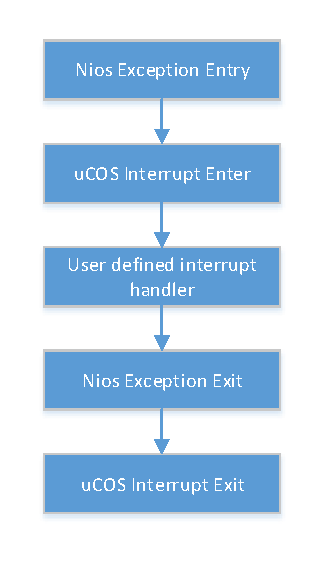
\includegraphics[scale=0.8]{Figures/exception_flow}
%\caption{Exception software flow in Nios II system.}
%\label{f:exception_flow}
%\end{figure}

\subsection{Fingerprint unit/Comparator Interface}
Messages are passed from the fingerprinting unit to the comparator when a task begins, when a fingerprint is complete, and when a task ends. The pausing of tasks is invisible to the comparator. Task begin/end messages can be sent in a single packet. Fingerprints require two packets to be sent to the comparator. The type of message being sent and the identity of the sender are encoded in the lower bits of the address. Table \ref{t:msg_format} shows the format for these messages. The size of each field could potentially be changed to satisfy different platform criteria. The messages could also be divided into two packets if the size of the offset becomes unreasonably large.
\begin{table}[h]
\centering
    \begin{tabular}{| l | l | l | l | l | }
    \hline
     & Base Address & Core ID & Message Type & Pad\\ \hline
    Message & 17 bits & 4 bits & 4 bits & 2 bits (0)\\ \hline
    \end{tabular}
    \caption{Message type format for sending messages from the fingerprint unit to the comparator.}
    \label{t:msg_format}
\end{table}
\begin{table}[ht]
\centering
    \begin{tabular}{| l | l |}
    \hline
    Message Type & Value\\ \hline
    Status update & 0\\ \hline
    Fingerprint & 4\\ \hline
    \end{tabular}
    \caption{Message type values for sending messages from the fingerprint unit to the comparator.}
    \label{t:msg_types}
\end{table}

The possible values for the current message types are shown in Table \ref{t:msg_types}. In the case of sending a fingerprint, it is necessary to break the 32 bit CRC up into two messages in order to be able to send the FID of the task that generated the fingerprint as well.  The format for sending fingerprints over two packets is shown in Table \ref{t:fprint_format}.

\begin{table}[h]
\centering
   \begin{tabular}{| l | l | l | l | }
    \hline
     & Partial Fingerprint & Packet & FID\\ \hline
    Lower half & 16 bits & 12b'0 & 4 bits\\ \hline
    Upper half & 16 bits & 12b'10 & 4 bits\\ \hline
    \end{tabular}
    \caption{Format for sending 32 bitfingerprints in 2 packets.}
    \label{t:fprint_format}
\end{table}


\subsection{Comparator/Monitor Interface}

Table \ref{t:comp_reg} contains the list of registers in the Comparator unit that can be accessed by the monitor core. The directory stores the offsets for start and end pointers of a circular queue and the addressing convention is given in Table \ref{t:dir_format}. The format for setting the core assignment table is shown in Table \ref{t:cat_format}. Each entry in the table is given by a unique address and addressing assumes that the size of the individual entry is 4 bytes even if the physical size of the memory is different (i.e. line 0 is at 0x0 and line 1 is at 0x4 regardless of the size of a line). Note that all address offsets are given from the perspective of the sender. The sender address offset is always shifted left by two bits compared to the offset the receiver uses.

The functions available to the monitor are:
\begin{itemize}
\item{fprint\_reset\_irq(void): Resets the status, fail and success register.} 
\item{set\_task\_directory(Directory\_Init\_Struct*): Set an entry of the directory.}
\item{fprint\_status(Fprint\_Status* fps): Retrieve the value of the three control registers.}
\item{set\_core\_assignment\_table(Core\_Assignment\_Table* ca): Sets the entire core assignment table.} 
\end{itemize}

\begin{table}
\centering
    \begin{tabular}{| l | l | l | p{8cm} |}
    \hline
    Register & RW & Offset & Function\\ \hline
    Status & RW & 0xC0 & Bit 6 is IRQ bit. Other bits reserved for future use.\\ \hline
    Success  & R & 0xC4 & Each bit of the success register is set to 1 when the corresponding task completes successfully. The register is automatically cleared when the status register is written to.\\ \hline
    Fail & R & 0xC8 & Each bit of the fail register is set to 1 when an error is detected in the corresponding task. The register is automatically cleared when the status register is written to.\\ \hline
    \end{tabular}
    \caption{Comparator control registers}
    \label{t:comp_reg}
\end{table}
\begin{table}
\centering
    \begin{tabular}{| l | l | l | l | p{6cm} |}
    \hline
    Name & RW & Offset & size & Function\\ \hline
    Start Pointer & W & 0x40 & 0x20 & Store the start pointers for each task: task 0 at offset x040, task 1 at offset 0x44, etc.\\ \hline
    End Pointer & W & 0x80 & 0x20 & Store the end pointers for each task: task 0 at offset x080, task 1 at offset 0x84, etc.\\ \hline
    \end{tabular}
    \caption{Comparator directory addressing format}
    \label{t:dir_format}
\end{table}

\begin{table}
\centering
    \begin{tabular}{| l | l | l | l |}
    \hline
    Address & VCID (1 bit) & Base Offset (6 bits) & Pad (2bits)\\ \hline
    Data & FID (4 bits) & PCID (4 bits) & Pad (2 bits)\\ \hline
    \end{tabular}
    \caption{Comparator Core Assignment table addressing and data format}
    \label{t:cat_format}
\end{table}

\section{Custom IP Microarchitectures}
This paper has taken a top-down approach in specifying the fingerprinting capable platform. First came a general overview of some important trends in dependable system design including two important examples: a reliable MPSoC and a hypervisor for partitioning of mixed critical systems. Following this, the software control flow was explored in greater detail in order to understand how fingerprinting services could be integrated into application or hypervisor code. This Chapter has so far covered the interfaces between each pair of agents in the system that are able to communicate with each other. A fairly complete \emph{black-box} description of the fingerprinting and comparator units has been established. It is now possible to examine the design of these peripherals at the register-transfer level.

\subsection{Fingerprint Unit}
There are three ports to the fingerprinting unit, as shown in Figure \ref{f:fprint_icon}. There is an addressable slave port for accessing the control registers, a port connected to the data bus directly (bypassing any bus translation and routing logic) used to calculate fingerprints, and a master port for sending information to the comparator.

Figure \ref{f:fprint_sch} shows the schematic for the fingerprint unit. The behaviour of the fingerprint unit is broken down into three independent FSMs. This will make future modifications to the pause or message passing protocols easier as they are independent of each other. Also, notice that the three variables stored in the fingerprinting unit, the FID, the counter value, and the fingerprint itself all have stacks associated with them. When a task is paused, the state of these three registers are pushed onto their respective tasks. Before the unpause strobe occurs, a new task can begin fingerprinting without corrupting the state of the previous task. The stack currently has a depth of eight. The LIFO structure is valid since we are only considering support for schedules with RM scheduling.


\begin{figure}[h]
\centering
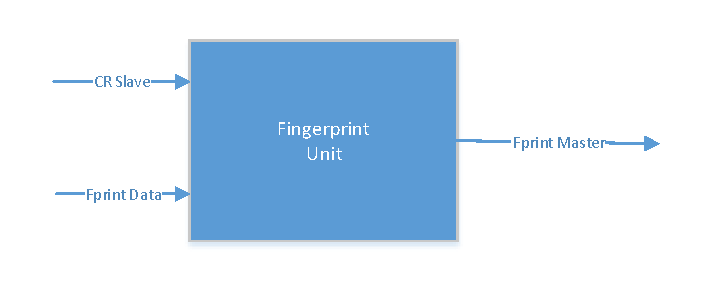
\includegraphics[scale=0.8]{Figures/fprint_icon}
\caption{Fingerprint unit ports.}
\label{f:fprint_icon}
\end{figure}

\begin{figure}[ht]
\centering
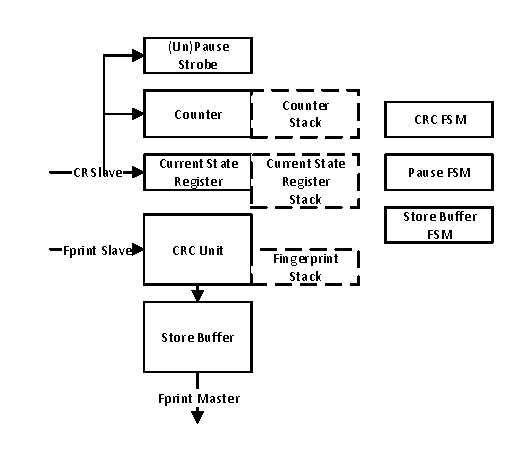
\includegraphics[width=10cm]{Figures/fprint_sch}
\caption{Schematic of the fingerprint unit components.}
\label{f:fprint_sch}
\end{figure}


\subsubsection{CRC Implementation}
The CRC implementation is shown in Figure \ref{f:crc}. A detailed explanation of how the CRC circuit is derived can be found in \cite{Hamed:12}. The circuit has been further modified to allow a \emph{variable} input data width. The implementation hinges on the RTLA multiplexers. For a $W$ bit circuit there will be $RTLA_i$ multiplexers indexed $1 < i < W$.
For an $M$ bit fingerprint, it is possible to shift the values in the RTLA to the right such that only the upper part of the circuit is used. This is useful for future implementations when load and store instructions will be used. For load instructions, only the address will be fingerprinted. By ensuring that the upper bits of the input $A_i$ are the address bits from the bus, it is possible to keep the block from being overly padded with zeros. In Figure \ref{f:rtla}, (a) shows the original RTLA while (b) and (c) show the updated RTLA capable of updating the fingerprint of either the address or the address and data inputs depending on whether or not the instruction is a store or a load. 

\begin{figure}[ht]
\centering
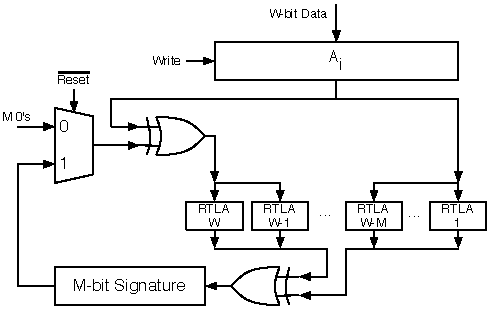
\includegraphics[width=10cm]{Figures/crc}
\caption{Implementation of CRC algorithm.}
\label{f:crc}
\end{figure}

\begin{figure}[ht]
\centering
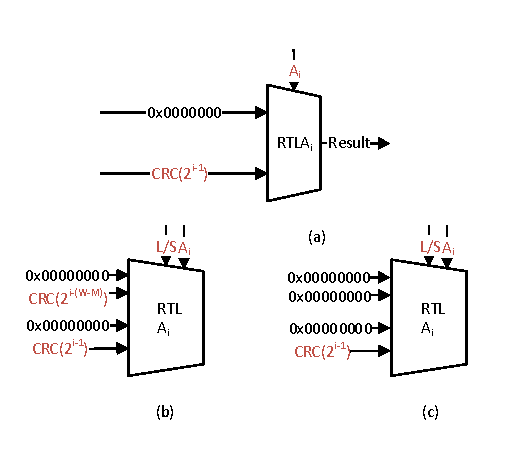
\includegraphics[scale=1]{Figures/rtla}
\caption[RTLA modification]{\emph{RTLA modification:} (a) original RTLA. (b) The RTLA for the upper portion of the input. When a load instruction is being fingerprinted the lower RTLA values are shifted right. (c) The lower portion of the input is completely deactivated during load instructions.}
\label{f:rtla}
\end{figure}

\subsubsection{Preventing state corruption during pause}
As was already discussed in Chapter \ref{Chapter2}, it is not possible to pause fingerprinting without causing at least one erroneous store instruction. Therefore each state register is doubled in order to store the \emph{previous} value to the latest calculation. It is the previous value that is pushed onto the stack to be restored when a task is unpaused. Furthermore, it is important to ensure that there are mechanisms to catch whether the erroneous store \emph{completes} a fingerprinting block. In the current implementation, the store buffer holds onto fingerprints until either a pause strobe or any other event occurs that changes state. The fingerprint is discarded if a pause strobe is the next event. Otherwise it is sent to the comparator. 

\subsection{Comparator}
The comparator collects fingerprints from all the cores in a system and compares them. The current implementation of the comparator is limited to 16 cores and two-way comparison. Ideas previously discussed in the interface sections as well as Chapter \ref{Chapter2} will receive less thorough treatment. Figure \ref{f:comp_sch} shows the comparator schematic with all the main components. Figure \ref{f:comp_fsm} shows the comparator FSM. The implementation of the comparator is quite involved and somewhat counter-intuitive and the best way to understand how it behaves as a whole is to directly examine the Verilog code. A summary of each state will be given. Three new data structures must first be introduced: the \emph{Fprint Trigger} register and the \emph{Checkin and Checkout} registers, and the \emph{Head and Tail Pointers}.

\begin{figure}[ht]
\centering
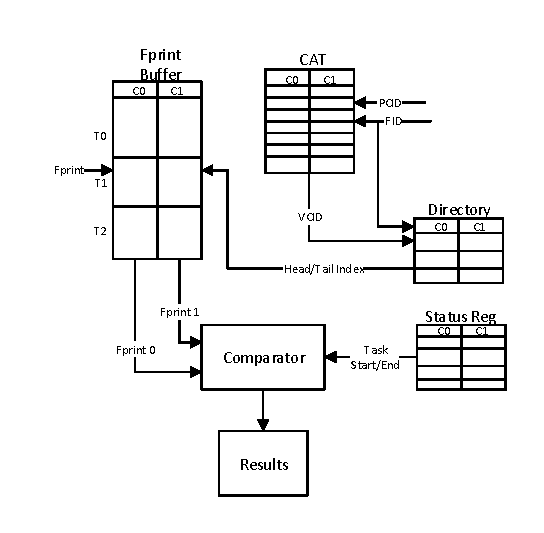
\includegraphics[scale=1.5]{Figures/compsch}
\caption[Comparator schematic]{\emph{Comparator schematic:} The FID, PCID and fingerprint arrive from the fingerprint unit. The FID and PCID are embedded in the address offset. The CAT is used to determine the VCID. The directory uses the VCID to locate the head pointer for the given FID. The comparator communicates with all the data structures but these signals have been omitted for clarity.}
\label{f:comp_sch}
\end{figure}
The \emph{Fprint Trigger} register keeps track of when the first new fingerprint arrives for a task since the last fingerprint was compared. This register is necessary because the arrival of a fingerprint is not in itself an event that should trigger comparison. Only once new fingerprints are available from both cores should a comparison be done. Also, in the case where a comparison cannot immediately be serviced, for instance if fingerprints arrive from several different tasks at once, the comparator can easily keep track of what is left to be done. The \emph{Checkin and Checkout} registers are simply registers that maintain a record of whether a task has started or ended on either of the virtual cores. The \emph{head and tail} registers keep track of the position of each task within the fingerprint queue. Remember that each task has its own start and end pointers that define a subset of the total fingerprint memory for a circular queue.

\begin{enumerate}
\item{\emph{Init:} The comparator is in an initial wait stage until an event occurs. Either a task has completed or a fingerprint has arrived.}
\item{\emph{Set Task:} The FID that caused the event is retrieved.}
\item{\emph{Load Pointer:} The tail pointer of the associated FID is loaded}
\item{\emph{Load Fprint:} The fingerprints are retrieved from the fingerprint buffer using the tail pointer.}
\item{\emph{Check Task Status:} If the checkin is activated for the given FID, then the task has completed(State 6). Otherwise proceed to State 7 to compare fingerprints.}
\item{\emph{Task Complete:} If the two head pointers match, then the same number of fingerprints arrived for both cores and the task was successful. Otherwise there was a problem (but no comparison took place because the comparator waits for new fingerprints from \emph{both} cores.}
\item{\emph{Compare Fprints:} If the fingerprints match then the tail pointer should be incremented (State  10). Otherwise a mismatch is detected.}
\item{\emph{Mismatch Detected:} An error has occurred.}
\item{\emph{Task Verified:} The task has been verified.}
\item{\emph{Increment Tail Pointer:} After a fingerprint comparison occurs, it is necessary to increment the tail pointer to proceed to the next comparison.}
\item{\emph{Check if Done:} This state checks whether for some reason several fingerprints were waiting to be compared, in which case the next comparison occurs. Otherwise the Fprint Trigger bit for the current FID is reset.}
\item{\emph{Reset Fprint Trigger:} Reset the Fprint Trigger bit for the current FID.}
\item{\emph{Reset Head and Tail:} The head and tail pointers for the given task should be reset when an error occurs.}
\item{\emph{Write Status Reg:} The status register should be updated and an interrupt will be sent to the Monitor. Further updates to status register can be made up until the monitor responds to the interrupt.}
\end{enumerate}




\begin{figure}[ht]
%\centering
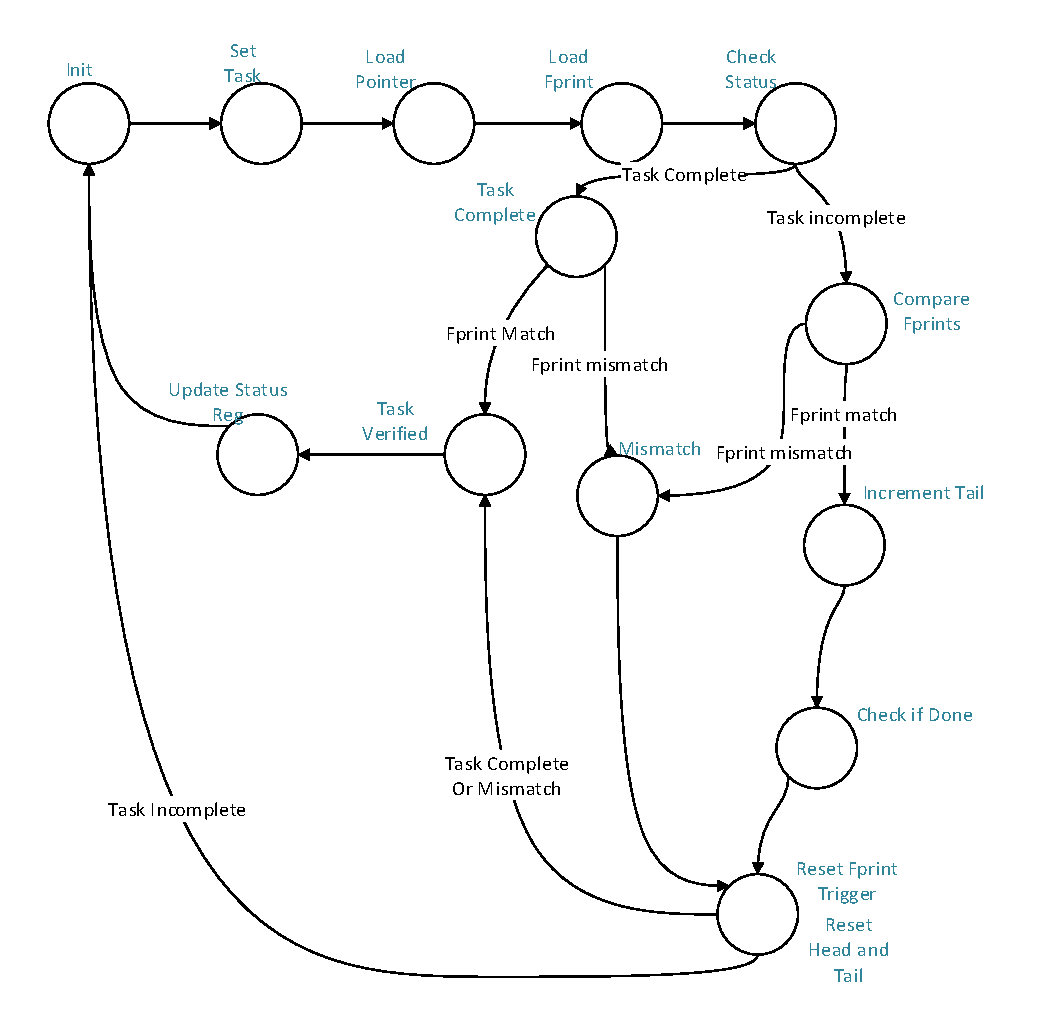
\includegraphics{Figures/comp_fsm}
\caption{Comparator FSM}
\label{f:comp_fsm}
\end{figure}


